% This file was created with tikzplotlib v0.10.1.
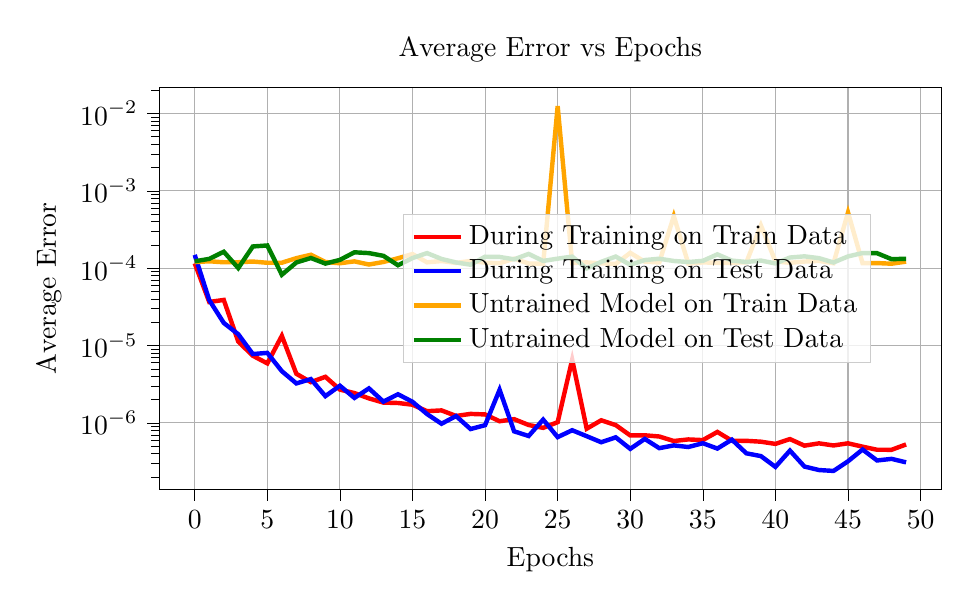
\begin{tikzpicture}

  \definecolor{darkgray176}{RGB}{176,176,176}
  \definecolor{green}{RGB}{0,128,0}
  \definecolor{lightgray204}{RGB}{204,204,204}
  \definecolor{orange}{RGB}{255,165,0}
  
  \begin{axis}[
    width = 0.95\textwidth,
    height = 19em,
  legend cell align={left},
  legend style={
    fill opacity=0.8,
    draw opacity=1,
    text opacity=1,
    at={(0.91,0.5)},
    anchor=east,
    draw=lightgray204
  },
  % log basis y={10},
  tick align=outside,
  tick pos=left,
  title={Average Error vs Epochs},
  x grid style={darkgray176},
  xlabel={Epochs},
  xmajorgrids,
  xmin=-2.45, xmax=51.45,
  xtick style={color=black},
  y grid style={darkgray176},
  ylabel={Average Error},
  ymajorgrids,
  ymin=1.3929386884171e-07, ymax=0.0214137849226391,
ymode=log,
ytick style={color=black},
ytick={1e-08,1e-07,1e-06,1e-05,0.0001,0.001,0.01,0.1,1},
yticklabels={
  \(\displaystyle {10^{-8}}\),
  \(\displaystyle {10^{-7}}\),
  \(\displaystyle {10^{-6}}\),
  \(\displaystyle {10^{-5}}\),
  \(\displaystyle {10^{-4}}\),
  \(\displaystyle {10^{-3}}\),
  \(\displaystyle {10^{-2}}\),
  \(\displaystyle {10^{-1}}\),
  \(\displaystyle {10^{0}}\)
}
]
\addplot [ultra thick, red]
table {%
0 0.000115619572170544
1 3.66140666301362e-05
2 3.88987718906719e-05
3 1.12463349069003e-05
4 7.39141842132085e-06
5 5.88246757615707e-06
6 1.33564672069042e-05
7 4.32045681009186e-06
8 3.36766470354632e-06
9 3.94663265979034e-06
10 2.69568681687815e-06
11 2.43232580032782e-06
12 2.07539164875925e-06
13 1.83115344043472e-06
14 1.81004190835665e-06
15 1.71904935086786e-06
16 1.41902387440496e-06
17 1.45171202348138e-06
18 1.23093161619181e-06
19 1.30822729715874e-06
20 1.28785870856518e-06
21 1.05134529349016e-06
22 1.11863823804015e-06
23 9.40535358040506e-07
24 8.63363482039858e-07
25 1.02263186363416e-06
26 6.57841155771166e-06
27 8.42167764858459e-07
28 1.08156234546186e-06
29 9.38011964990437e-07
30 6.88994134634413e-07
31 6.92170203819842e-07
32 6.67649260321923e-07
33 5.83880023441452e-07
34 6.11951520568255e-07
35 6.00160205976863e-07
36 7.64876006087434e-07
37 5.89186356592108e-07
38 5.87023293974198e-07
39 5.72065005144395e-07
40 5.35504113940988e-07
41 6.18023648257804e-07
42 5.08474954585836e-07
43 5.44603835805901e-07
44 5.11379028012016e-07
45 5.45023794984445e-07
46 4.93479035412747e-07
47 4.499693204707e-07
48 4.4950027699997e-07
49 5.27288420926197e-07
};
\addlegendentry{During Training on Train Data}
\addplot [ultra thick, blue]
table {%
0 0.000148638486280106
1 3.8717822462786e-05
2 1.96167875401443e-05
3 1.40024994834675e-05
4 7.77251534600509e-06
5 8.04341743787518e-06
6 4.66747496830067e-06
7 3.24275606544688e-06
8 3.68673295270128e-06
9 2.22127937377081e-06
10 3.02577313959773e-06
11 2.10539269573928e-06
12 2.79613914244692e-06
13 1.88535034340021e-06
14 2.34871004067827e-06
15 1.87500120318873e-06
16 1.30373712181608e-06
17 9.7612542049319e-07
18 1.22695689697139e-06
19 8.33635738217708e-07
20 9.3538966439155e-07
21 2.68304006567632e-06
22 7.79187587340857e-07
23 6.77797231674049e-07
24 1.10359292193607e-06
25 6.55734368137928e-07
26 8.04333865289664e-07
27 6.73910278692347e-07
28 5.62983984764287e-07
29 6.51476170787646e-07
30 4.62268644696451e-07
31 6.21099786712875e-07
32 4.7201328357005e-07
33 5.12390784024319e-07
34 4.88249042973621e-07
35 5.46861258499121e-07
36 4.66291567136068e-07
37 6.0789801636929e-07
38 4.04685039256947e-07
39 3.72652806390761e-07
40 2.70373163857585e-07
41 4.39054105072501e-07
42 2.73006207862636e-07
43 2.46051911290124e-07
44 2.39714267991076e-07
45 3.1927794452713e-07
46 4.52996403055295e-07
47 3.27289853885304e-07
48 3.43154766824227e-07
49 3.09403873188785e-07
};
\addlegendentry{During Training on Test Data}
\addplot [ultra thick, orange]
table {%
0 0.000119844757136889
1 0.000122850964544341
2 0.000119242758955806
3 0.0001194120341097
4 0.000121909339213744
5 0.000117509182018694
6 0.000117711497296114
7 0.000134808011353016
8 0.000149091443745419
9 0.000120183576655108
10 0.000115898626972921
11 0.000122511555673555
12 0.000111565263068769
13 0.000120325428724755
14 0.000134350819280371
15 0.000152338034240529
16 0.000119035270472523
17 0.00012379974941723
18 0.000117030824185349
19 0.000124024198157713
20 0.000117830757517368
21 0.000115914219350088
22 0.00013274562661536
23 0.00011486293078633
24 0.000114014488644898
25 0.0124431848526001
26 0.000116647170216311
27 0.000118882482638583
28 0.000115469163574744
29 0.000113608708488755
30 0.00015779300883878
31 0.000121383927762508
32 0.000118668504001107
33 0.00047049461863935
34 0.000114619404484984
35 0.00011880121746799
36 0.000117411691462621
37 0.000117397568828892
38 0.000119214426376857
39 0.000357582262950018
40 0.000122612778795883
41 0.000117423463962041
42 0.000121910503366962
43 0.000124323123600334
44 0.000115912305773236
45 0.000524870993103832
46 0.000116180184704717
47 0.000116481249278877
48 0.000114282163849566
49 0.000121571094496176
};
\addlegendentry{Untrained Model on Train Data}
\addplot [ultra thick, green]
table {%
0 0.000122817582450807
1 0.000132000757730566
2 0.000163245917065069
3 0.000100329452834558
4 0.000190929204109125
5 0.000196753637283109
6 8.23061054688878e-05
7 0.000118566029414069
8 0.000135401103761978
9 0.000114686314191204
10 0.000128131257952191
11 0.000160483745275997
12 0.000156743626575917
13 0.000144422388984822
14 0.00010919920168817
15 0.000135145717649721
16 0.000156790585606359
17 0.000131657448946498
18 0.000118700903840363
19 0.000110858003608882
20 0.00014075958461035
21 0.000139842843054794
22 0.000130170141346753
23 0.000152905340655707
24 0.000124135913210921
25 0.000132893052068539
26 0.000141130716656335
27 9.90790795185603e-05
28 0.000120807693747338
29 0.000141456825076602
30 0.000110587214294355
31 0.000127455787151121
32 0.00013254517398309
33 0.00012397175305523
34 0.000120144453831017
35 0.000124459431390278
36 0.000150959225720726
37 0.000125301812659018
38 0.000120412958494853
39 0.000125558653962798
40 0.000115242255560588
41 0.000137347829877399
42 0.000142319564474747
43 0.000134914516820572
44 0.000118584044685122
45 0.000142000455525704
46 0.000157046873937361
47 0.000156261696247384
48 0.000130856220494024
49 0.000132377448608167
};
\addlegendentry{Untrained Model on Test Data}
\end{axis}

\end{tikzpicture}
